\documentclass[conference]{IEEEtran}
\IEEEoverridecommandlockouts
% The preceding line is only needed to identify funding in the first footnote. If that is unneeded, please comment it out.
\usepackage{cite}
\usepackage{amsmath,amssymb,amsfonts}
\usepackage{algorithmic}
\usepackage{textcomp}
\usepackage{theorem,caption,extarrows,mathrsfs,physics,bm}
\usepackage{graphicx,xcolor,booktabs,subfigure,tikz}
\usepackage{pgfplots,grffile}
\usepackage{fontspec,xeCJK}
\setmainfont{TeX Gyre Termes}
\usepackage[skins]{tcolorbox}
\usepackage{listings}
\lstset{
    basicstyle          =   \sffamily,          % 基本代码风格
    keywordstyle        =   \bfseries,          % 关键字风格
    commentstyle        =   \rmfamily\itshape,  % 注释的风格,斜体
    stringstyle         =   \ttfamily,  % 字符串风格
    flexiblecolumns,                % 别问为什么,加上这个
    numbers             =   left,   % 行号的位置在左边
    showspaces          =   false,  % 是否显示空格,显示了有点乱,所以不现实了
    numberstyle         =   \tiny\ttfamily,    % 行号的样式,小五号,tt等宽字体
    showstringspaces    =   false,
    captionpos          =   t,      % 这段代码的名字所呈现的位置,t指的是top上面
    frame               =   shadowbox,   % 显示边框
    rulesepcolor=\color{red!20!green!20!blue!20}
}

\lstdefinestyle{Python}{
    language        =   Python, % 语言选Python
    backgroundcolor=\color{backpycol},
    basicstyle      =   \ttfamily,
    numberstyle     =   \ttfamily,
    keywordstyle    =   \color{blue},
    keywordstyle    =   [2] \color{teal},
    stringstyle     =   \color{magenta},
    commentstyle    =   \color[HTML]{338AAF}\ttfamily,
    breaklines      =   true,   % 自动换行,建议不要写太长的行
    columns         =   fixed,  % 如果不加这一句,字间距就不固定,很丑,必须加
    basewidth       =   0.5em,
}
\definecolor{codegreen}{rgb}{0,0.6,0}
\definecolor{codegray}{rgb}{0.5,0.5,0.5}
\definecolor{codepurple}{rgb}{0.58,0,0.82}
\definecolor{backcolour}{rgb}{0.95,0.95,0.92}
\definecolor{backpycol}{rgb}{0.97,0.95,0.97}
\lstdefinestyle{C++}{
    language =[ANSI]C,
    backgroundcolor=\color{backcolour},
    commentstyle=\color[HTML]{338AAF}\ttfamily,
    keywordstyle=\sffamily\bfseries\color{magenta},
    numberstyle=\color{codegray},
    stringstyle=\color{codepurple},
    basicstyle=\ttfamily,
    breakatwhitespace=false,
    breaklines=true,
    basewidth=0.5em,
    captionpos=b,
    columns=fixed,
    frame=shadowbox,
    keepspaces=true,
    numbers=left,
    numbersep=5pt,
    showspaces=false,
    showstringspaces=false,
    showtabs=false,
    tabsize=4
}
\lstdefinestyle{matlab}{
    language=matlab,
    backgroundcolor=\color{backcolour},
    commentstyle=\color[HTML]{338AAF}\ttfamily,
    keywordstyle=\sffamily\bfseries\color{magenta},
    numberstyle=\color{codegray},
    stringstyle=\color{codepurple},
    basicstyle=\ttfamily,
    breakatwhitespace=false,
    breaklines=true,
    basewidth=0.5em,
    captionpos=b,
    columns=fixed,
    keepspaces=true,
    numbers=left,
    numbersep=5pt,
    showspaces=false,
    showstringspaces=false,
    showtabs=false,
    tabsize=4,
    frame=shadowbox
}
\definecolor{mygreen}{rgb}{0,0.6,0}
\definecolor{mygray}{rgb}{0.5,0.5,0.5}
\definecolor{mymauve}{rgb}{0.58,0,0.82}
\definecolor{bggray}{rgb}{0.93,0.95,0.94}
\lstdefinestyle{pseudocode}{
    backgroundcolor=\color{bggray},
    columns=fullflexible,
    tabsize=4,
    breaklines=true,               % automatic line breaking only at whitespace
    captionpos=b,                  % sets the caption-position to bottom
    commentstyle=\color{mygreen},  % comment style
    escapeinside={\%*}{*)},        % if you want to add LaTeX within your code
    keywordstyle=\color{blue},     % keyword style
    stringstyle=\color{mymauve}\ttfamily,  % string literal style
    frame=shadowbox,
    rulesepcolor=\color{red!20!green!20!blue!20},
    % identifierstyle=\color{red},
    language=c++,
    numbers=left,
    numberstyle=\small\color{codegray},
    basicstyle=\ttfamily,% size of fonts used for the code
    escapeinside=``,
    xleftmargin=0.6em,
    xrightmargin=0.6em,
    aboveskip=1em
}
\lstdefinestyle{Fortran}{
    language =fortran,
    backgroundcolor=\color{backcolour},
    commentstyle=\color[HTML]{338AAF}\ttfamily,
    keywordstyle=\sffamily\bfseries\color{magenta},
    numberstyle=\small\color{codegray},
    stringstyle=\color{codepurple},
    basicstyle=\ttfamily,
    breakatwhitespace=false,
    breaklines=true,
    basewidth=0.5em,
    captionpos=b,
    columns=fixed,
    frame=shadowbox,
    keepspaces=true,
    numbers=left,
    numbersep=5pt,
    showspaces=false,
    showstringspaces=false,
    showtabs=false,
    tabsize=4
}
\setmonofont{CMU Typewriter Text}
\pgfplotsset{compat=newest}
  %% the following commands are needed for some matlab2tikz features
\usetikzlibrary{plotmarks}
\usetikzlibrary{arrows.meta}
\usetikzlibrary{calc}
\usepgfplotslibrary{patchplots}
\def\BibTeX{{\rm B\kern-.05em{\sc i\kern-.025em b}\kern-.08em
    T\kern-.1667em\lower.7ex\hbox{E}\kern-.125emX}}
%% Define the theorem and proof
\newtheorem{theorem}[subsection]{Theorem}
\newtheorem{definition}[subsection]{Definition}
\newenvironment{thmbox}{\par
	\vspace{4pt}
	\begin{center}
	\tcbset{enhanced,notitle,colframe=black,colback=white}
	\begin{tcolorbox}[fuzzy shadow={1.6mm}{-1.6mm}{0mm}{0mm}{fill=black!90!white},arc=0mm]}{\end{tcolorbox}
	\end{center}}
\begin{document}
\title{Mini-project: MATLAB-based Piano Sound Synthesis}
\author{
	\IEEEauthorblockN{1\textsuperscript{st} Qiu Kunyuan}
	\IEEEauthorblockA{
		\textit{EEE. Southern University of Science and Technology}\\
		Shenzhen, PRC\\
		11913019@mail.sustech.edu.cn
	}
}
\maketitle
\begin{abstract}
	In this paper, the advantages and disadvantages of various sound simulation techniques have been analyzed, and then a method for synthesizing piano sounds using ADSR model and string vibration model has been implemented based on the previous work\cite{css_piano}\cite{cmf_piano}.

	This method simulates the physical properties of piano string vibration\cite{piano_model_ljs}\cite{piano_model_yz} and resonance box by MATLAB, and then generates the tones with overtones of various orders by using the string vibration law, and then modifies the string vibration tones according to the amplitude envelope and spectral envelope of the piano sound collected, and generates the syllables with specific duration and timbre.

	In this work, the proposed synthesis system is experimentally validated, and it is shown that the synthesized notes are harmonious, and the timbre performance is excellent, and the generated timbre characteristics can be flexibly changed, and the synthesized sound is close to various real instruments.
\end{abstract}

\begin{IEEEkeywords}
	sound simulation, ADSR model, string vibration, MATLAB
\end{IEEEkeywords}

\section{Introduction: Music Theory Expressed in Physics}
Music is an art made up of sound, and sound is a sound wave that can be perceived by the human ear. Sound signals with a specific frequency spectrum and amplitude envelope can stimulate the human auditory organs and bring aesthetic experiences to humans, and music is formed when humans generate such sound signals on their subjective initiative.

\subsection{Octaves and Frequency Response of Human Ears}
The primary acoustic characteristics that determine the human auditory experience are pitch and intensity. Pitch is the central frequency of the acoustic signal, and intensity is the amplitude of the acoustic signal.

Such rule of human acoustic response is firstly concluded and expressed by the A. Bach and other classic musicians like L. Beethoven and Hayton. It can be said that all the European classic music are based on the mathematical conclusions and empirical formulas with no exaggeration.

Since the linear distance from the top of the cochlear basilar membrane to the maximum displacement is proportional to the logarithm of the input frequency, and the output signal of the human auditory nerve is proportional to the logarithm of the sound pressure, the frequency response of the human auditory system follows a double logarithmic coordinate:

\begin{equation}
	p=\log(\frac{f}{f_{0}}),B=10\log(\frac{W}{W_0})
\end{equation}

For every doubling or doubling of frequency, the pitch rises by one unit, and this unit is called an octave. The average person can hear sounds from 20 to 20,000 Hz, and using 440 Hz, the most sensitive frequency in the human ear, as a reference, the human ear can hear about

\begin{equation}
	\left\lceil \frac{\log(\frac{f_min}{440})}{\log(2)} \right\rceil=-4, \left\lfloor \frac{\log(\frac{f_max}{440})}{\log(2)} \right\rfloor=5
\end{equation}

octaves below and above.

\subsection{Temperament and Key Scale}
Within an octave, the more sensitive sound frequencies of the human ear are concentrated in eight frequency points, and the ratio of two of these frequency points is a specific value of one or two squares.

Let \(q\) is the minimal frequency ratio between one note and the other, then an octave can be divided into 8 frequency points including 2 minor gaps and 5 major gaps that the frequency ratio of which is \(q^{2}\). Therefore, the ratio satisfies
\begin{equation}
	q^{2}\cdot (q^ {2})^ {5}=2\Rightarrow q=2^{1/12}
\end{equation}

Using this ratio and the gap relation, it is convenient to determine the frequency of arbitrary note inside an octave with the base frequency \(f_{0}\) given.
\begin{equation}
	f[k]=f_{0}q^{k}=f_{0}2^{\frac{k}{12}}
\end{equation}

In actual musical composing, it is a convention that the C1 note at 523Hz is used to determine the base frequencies,
\begin{equation}
	f_{0}[k]=f_{\text{C1}}2^{\frac{k}{12}}
\end{equation}

and the gap sequence
\begin{equation}
	k=[0,2,4,5,7,9,11]
\end{equation}

is conventionally referred to as the major scale. Therefore, an arbitrary major scale can be expressed as the formula below by substituting (1) and (5) into (4):
\begin{equation}
	f[k]=f_{C1}2^{(k_{0}+k)/12+p}
\end{equation}

Where
\begin{equation}
	p\in[-4,5],\{k_{0},k\}\subset\{0,2,4,5,7,9,11\}
\end{equation}

\subsection{Tone-color and Sounding Model of Piano String}
The subjective features of a musical tone other than its pitch, intensity and length is concluded as the tone-color, which is mostly determined by the frequency spectrum and the amplitude envelope of the sounding instrument.

Most mechanical oscillating bodies in the real world produces fading non-harmonic sound wave after a single excitation. For the sounding strings in the piano, the oscillation models under idealistic conditions can be theoretically derived by solving the 1-dimensional Helmholtz equation.
\begin{equation}
	\begin{cases}
		u_{tt}+\mu u_{t}  & =v^{2}u_{xx},                                                                               \\
		u|_{x=0}=u|_{x=l} & =0,                                                                                         \\
		u|_{t=0}          & =0,                                                                                         \\
		u_{t}|_{t=0}      & =\text{rect}\left( \frac{x-x_{0}}{2d} \right)v_{0}\cos\left( \pi \frac{x-x_{0}}{2d} \right)
	\end{cases}
\end{equation}

Solving this equation by variable separation method gives that
\begin{equation}
	\begin{cases}
		u(x,t)   & =A\exp(-\mu/2 t) \sum_{n=1}^{\infty} \frac{1}{n}\frac{1}{1-4d^2n^2/l^2}B(n,x,t), \\
		B(n,x,t) & =C_{n}\sin(n\pi x_{0}/l)sin(n\omega_0 t)                                         \\
		         & +D_{n}\cos(n\pi x_{0}/l)\cos(n\omega_0 t)
	\end{cases}
\end{equation}

The coefficients \(C_{n}, D_{n}\) in this solution is very hard to express analytically and requires experimental testing or manually adjusting. These coefficients are amplitudes of the harmonic components, and the combination of the coefficients partially controls the tone-color of the piano.

\subsection{ADSR Envelope Model of the Resonance Chamber}
The abundant tone-color and the time domain features of piano sound is determined not only by the excite signal from the oscillating strings, but also by the filter formed by the resonating chamber:
\begin{equation}
	y(t)=h_{\text{chamber}}(t)*\sum_{n=1}^{N} e_{n}(t)
\end{equation}

The effect of the resonating chamber normally results in echoing of the syllables that are simultaneously stroke and the dragging after the key is released. And the large volume of the typically wooden chamber attenuates the non-resonant frequency components produced by the string, while enabling the resonant frequency pass through. Thus, the resonating chamber can be modeled as a FIR filter with non-zero delay and more than 1 pass bands.

Taking into account the damping of the piano string and the impulse response of the resonant cavity, the piano tone also has a changing amplitude envelope in the time domain. Such envelope is characterized by a large initial value, a slow decay of the amplitude, and then a rapid decay to zero.

\begin{figure}[htpb]
	\centering
	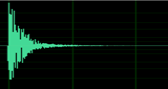
\includegraphics[width=0.43\textwidth]{adsr_real_piano.png}
	\caption{Real envelope of Piano Sound}
	\label{fig:adsr_real_piano.png}
\end{figure}

In the field of electronic musical instruments, the ADSR model, an empirical polyline model, can be used to provide a good approximation of the amplitude envelope of various musical tones.

\begin{figure}[htpb]
	\centering
	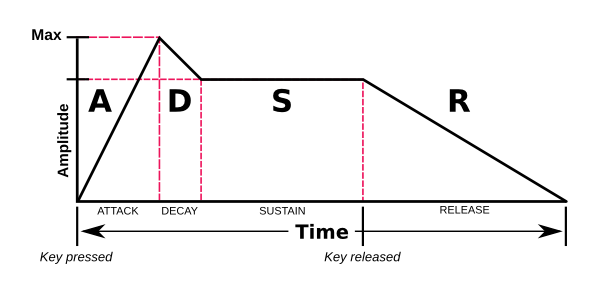
\includegraphics[width=0.43\textwidth]{adsr_concep.png}
	\caption{The Main Conception of ADSR Envelope}
	\label{fig:adsr_concep.png}
\end{figure}

\section{Synthesizer Design}

With the analysis above on the sounding progress of piano, there is no theoretical difficulty in forming the architecture of the synthesizer program. The simulator is divided into the tone generator, envelope modulator and echoing filter, since the sounding process in a real piano is composed by striking the string and echoing in the resonance chamber.

\begin{figure}[htpb]
	\centering
	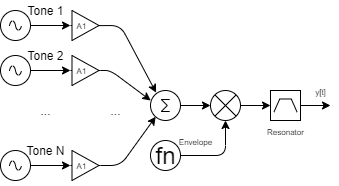
\includegraphics[width=0.43\textwidth]{synth_arch.png}
	\caption{Architecture of the Synthesizer}
	\label{fig:synth_arch.png}
\end{figure}

\subsection{Tone Generation and Synthesis}
In the string oscillation equation (10), the base frequency \( \omega_{0}  \) are injected from the note parameters in the simplified stave as the equation (7) and (8).

Let the
\begin{equation}
	l=[0,2,4,5,7,9,11]
\end{equation}
denotes the relative pitch sequence of arbitrary major scale, this list injects the pitch name
\begin{equation}
	k=[1:7]
\end{equation}
to the relative interval. For a scale consisting a tonic keynote \( l[k_{0}]  \), a conventional pitch name sequence \( l[k] \)  and an octave number \( p \) , the frequency of each note is obtained by deduction from the (7) and (8):
\begin{equation}
	f[k]=f_{C1}2^{(l[k_{0}]+l[k]+\Delta)/12+p}
\end{equation}

Where
\begin{equation}
	p\in[-4,5],\Delta =\{-1,0,1\}
\end{equation}
and the
\begin{equation}
	f_{C1}=523.2511 \text{Hz}, f_{A1}=440\text{Hz}
\end{equation}
is the absolute baseline that determines the absolute pitch or frequency.

Therefore, the function \lstinline{tone2freq(tone,noctave,rising)} and \lstinline{gen_wave(tone,scale,noctave,rising,rhythm,fs)} that evaluates the fundamental tone of a given note can be programmed easily by directly translating the formulas above to MATLAB code:

\paragraph{tone2freq.m}~{}

\lstinputlisting[language=matlab,style=matlab]{../matlab/tone2freq.m}

\paragraph{ToScale.m}~{}

\lstinputlisting[language=matlab,style=matlab]{../matlab/ToScale.m}

\subsection{Harmonic Overtone Synthesizing}
With the fundamental tone(frequency) deduced from pitch name in the section (A), the sound wave produced by the oscillation of the piano string can be determined in the frequency domain. The solution of 1-dimension Helmholtz equation states that the vibration waveform of a string is a periodic function expressed in Fourier series as (10):
\begin{equation}
	\begin{aligned}
		u(x,t)[k] & =A\exp(-\mu t/2)\sum_{n=1}^{\infty} P_{n}(B_{n}\exp(j n 2 \pi f[k]) \\
		          & +C_{n}\exp(-j n 2 \pi f[k]))
	\end{aligned}
\end{equation}

Where the \(f[k]\) is the fundamental frequency evaluated above from the pitch name, and the \(A,\mu ,B_{n},C_{n}\) are the empirical amplitude coefficients and damping coefficients measured by experiment. The commom coefficient
\begin{equation}
	P_{n}=\frac{1}{n}\frac{1}{1-4d^2n^2/l^2}
\end{equation}
is the common part of the sine and cosine terms in the solution, which indicates the amplitude decreasing along with the increase of mode order.

The far-field radiation pattern of the string is approximately cylindrical symmetric, similar to that of a dipole. This effect is neither dispersive nor time-varying, thus the effect of far-field radiation can be aggregated with the effect of the resonance chamber and treated as a BPF after.

The amplitude coefficients \(B_{n},C_{n}\) has already been measured experimentally in the existing research \cite{cmf_piano} and \cite{css_piano}. With the help of these two existing research, the highest harmonic order is chosen empirically as the formula below:
\begin{equation}
	N_{max}=\left\lceil \frac{f_{A1}\times N_{A1}}{f[k]} \right\rceil
\end{equation}

where the \(N_{A1}\) is the highest order that has significant effect(>30dB) to the synthesized tone color:
\begin{equation}
	\frac{B^{2}[N_{A1}]+C^{2}[N_{A1}]}{\sum(B_{n}^{2}+C_{n}^{2})}\lvert_{440\text{Hz}}>30\text{dB}
\end{equation}

All the deductions above leads to the waveform generation code below:
\begin{lstlisting}[language=matlab,style=matlab]
	fc1=tone2freq(note(1),note(2),note(3),key,0);
    fc1_list=fc1*(1:19);
    amp=[987.8,368.6,620.2,483.9,156.7,...
		83.62,120.1,70.73,5.348,24.41,...
		27.35,21.3,10.31,6.477,15.91,...
		3.495,2.546,0.4751,0.8858]/1000;
    wfm1=cell2mat(arrayfun(@(a,x) a*sin(2*pi*x*Tv),amp,fc1_list,'UniformOutput',false).');
\end{lstlisting}

\subsection{Resonance Chamber and ADSR Enveloping}
The frequency generator mentioned above generates a continuous signal that is almost constant in amplitude. Considering the damped vibration of the strings, the quadratic inverse attenuation of the sound waves in the air and the filtering of the resonance box together, the musical signal from the piano should have an ADSR envelope in the time domain and several concentrated resonance bands in the frequency domain.

The research~\cite{cmf_piano}~\cite{css_piano} both give out the experimentally measured envelopes in terms of piecewise function, and \cite{css_piano} also measured the resonance bands of the resonant box of a piano. The enveloping and filtering functions can be programmed with referencing to the two achievements above therefore.

\begin{lstlisting}[language=matlab,style=matlab]
	% Enveloping and Filtering
    wfm1=sum(wfm1,1).*GenADSRenv(wfm1,[0.008,0.09,0.11,0.25,0.67],...
	[0.88,0.88,0.56,0.50,0]);
    [b_b1,a_b1]=butter(6,2*[1300,1900]/Fs);
    [b_b2,a_b2]=butter(6,2*[3600,5000]/Fs);
    [b_b3,a_b3]=butter(6,2*[7800,8200]/Fs);
    wfm2=1.1*wfm1+0.4*filter(b_b1,a_b1,wfm1)+0.35*filter(b_b2,a_b2,wfm1)+0.25*filter(b_b3,a_b3,wfm1);
    wfm2=wfm2/(max(wfm2));
\end{lstlisting}

The expression of piecewise linear ADSR envelopes can be easily obtained by concatenating line sections in terms of two-point equation.
\begin{equation}
	\begin{aligned}
		y_{ADSR}[n] & =\sum_{0}^{N_{C}} \left( y_{C}[k]+nF_{S}\frac{y_{C}[k+1]-y_{C}[k]}{x_{C}[k+1]-x_{C}[k]} \right) \\
		            & \quad \times ((u(n-x[k+1]F_{S})-u(n-x[k]F_{S})))
	\end{aligned}
\end{equation}
where the vector
\begin{equation}
	\begin{pmatrix}
		x_{C}[n] \\
		y_{C}[n]
	\end{pmatrix}=
	\begin{pmatrix}
		y_{C}[0],\ldots,y_{C}[N_{C}] \\
		x_{C}[0],\ldots,x_{C}[N_{C}] \\
	\end{pmatrix}
\end{equation}
are the time and amplitude of the control points \(x_{C}[n]=(x_{1},x_{2},\ldots,x_{n})\) and \(y_{C}[n]=(y_{1},y_{2},\ldots,y_{n})\), and \(F_{S}\) is the sampling frequency corresponding to the input soundwave.

\subsection{Score File Reading}
In order to decouple the score data from the player and enhance the user-friendliness of the program, a separate text file is used to record the key signature, the beat, the sample rate and the score. By separating the score from the player, it is also convenient for users to compose their own scores for playing custom tracks, as well as enabling future extensions such as multitracking.

The capability of reading the score is implemented through \lstinline[language=matlab]{fscanf()} function, which is a MATLAB built-in function.

\lstinputlisting[language=matlab,style=matlab]{../matlab/PlayMusicFile.m}

The format of an example score file is shown below. The first row of the score contains the base key, rhythm speed and sampling frequency in Hertz, and the succeeding rows consist of the 4 elementary data of a note, respectively the tone, number of octave, quarter rising and sustaining time.

\begin{lstlisting}[style=matlab]
	D 76 Fs=48000
	6 0 0 0.5
	7 0 0 0.5
	1 1 0 1.5
	7 0 0 0.5
\end{lstlisting}

\section{Extension on Symphony}

A symphony is composed by a couple of different soundtracks playing simultaneously, and the harmonic mixing of such individual waveforms in a resonating chamber creates grand music experience with sacred feeling. For MATLAB based synthesizer, such symphony can be easily realized by using multiple synthesizers configured to emulate different musical instruments, and then use a mixer with the frequency response of the Golden Hall or any other music halls.

With this technique, the synthesizer mentioned above can be used to play the classic Germany and Austrian symphonies composed in the 19th to early 20th centuries.


%references
\bibliographystyle{IEEEtran}
\bibliography{reference.bib}


\end{document}